\chapter{Reinforcement Learning}

\begin{figure}[ht]
    \centering
    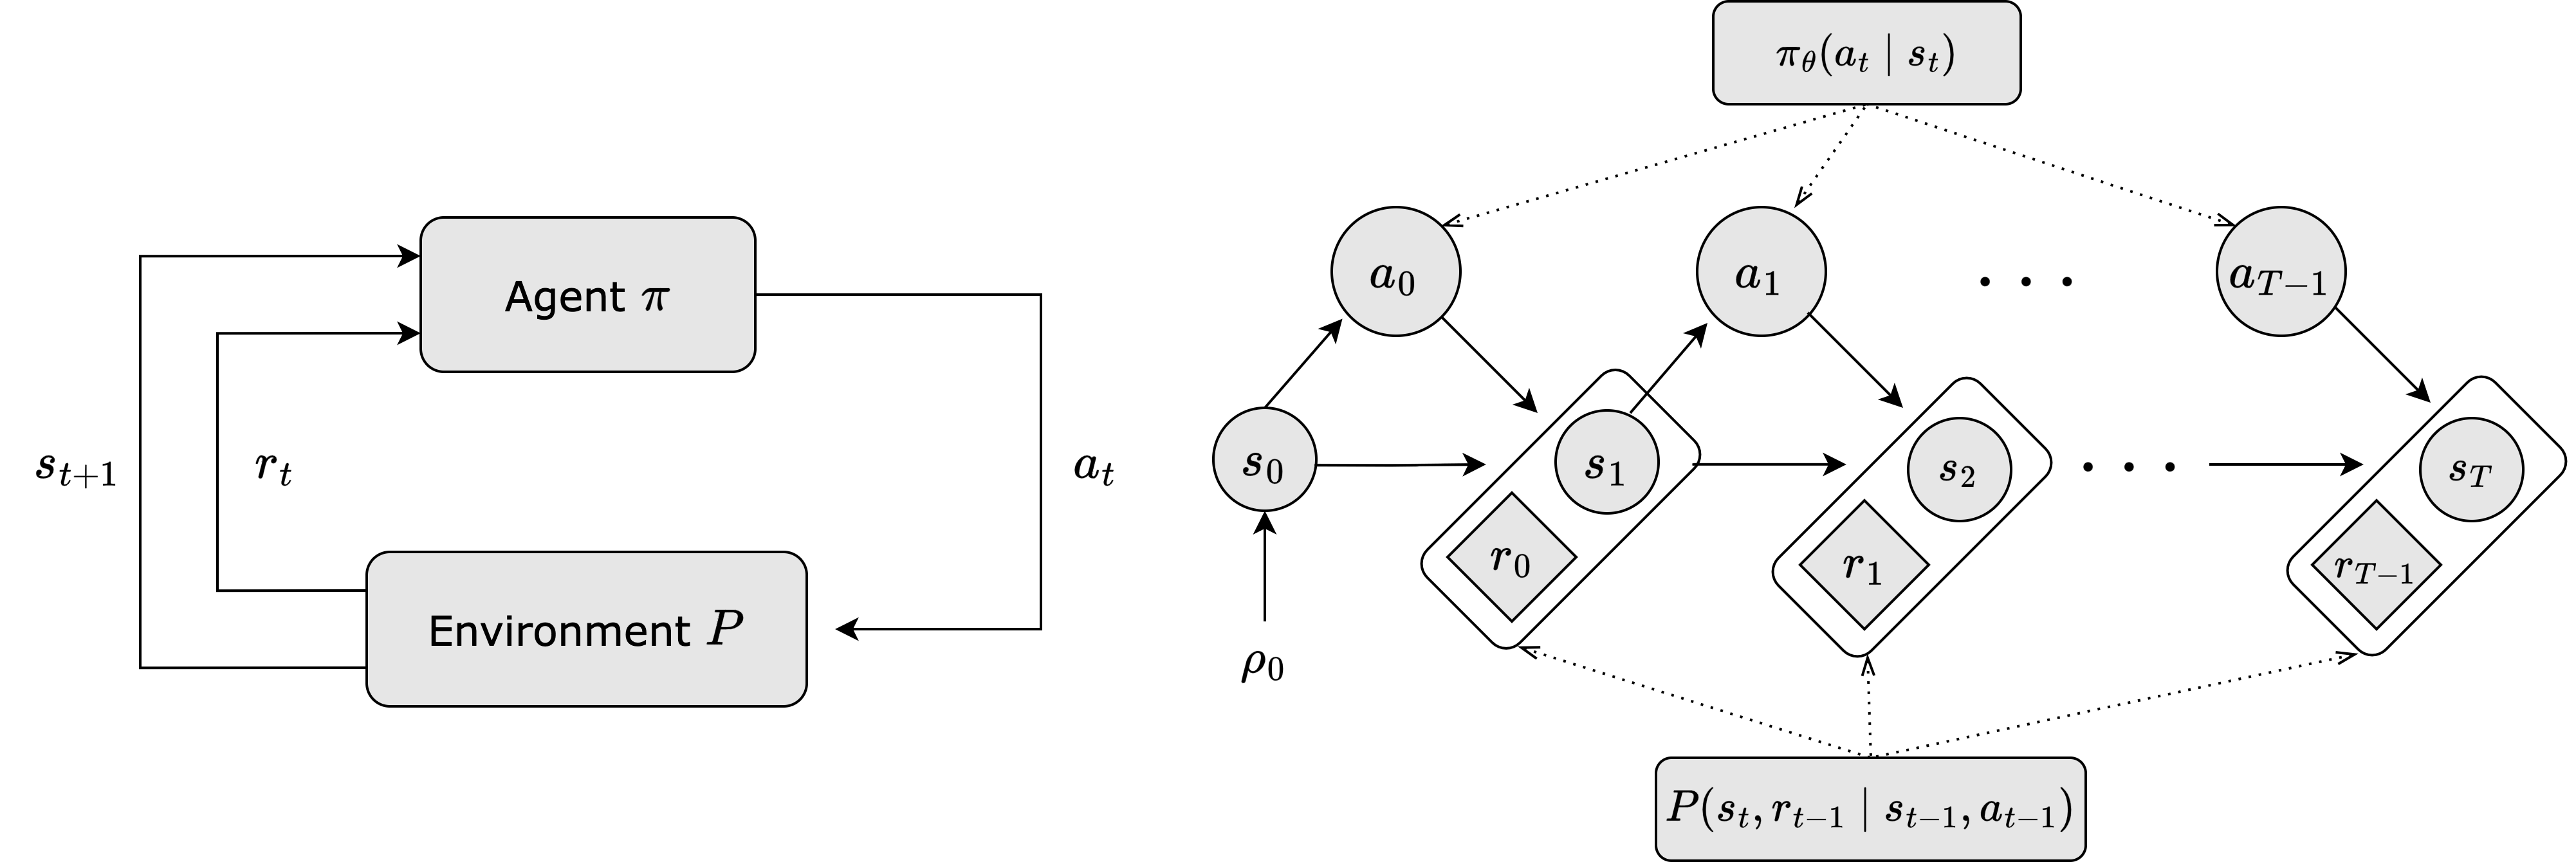
\includegraphics[scale=0.65]{ch3-rl/MDP-diagram.png}
    \captionsetup{width=\textwidth} % set the width of the caption
    \caption{\textbf{Left:} A loop representation of a Markov Decision Process (MDP). \textbf{Right:} An unrolled MDP depecting an episodic case with a finite horizon $T$ and a parameterized policy $\pi_{\theta}$.}
    \label{fig:mdp-diagram}
  \end{figure}

Reinforcement learning (RL) is all about the interaction between an agent and the environment. The learning comes in the form of trial-and-error, in which the agent observe the state of the environment, takes actions according to that observations, influencing new possible states configurations, and perceive rewards given its previous decision. Everything is commanded toward achieve a goal such as escaping from a maze, \href{https://arxiv.org/abs/1312.5602}{win some Atari Game} \citep{mnih2013playing}, or \href{https://deepmind.google/technologies/alphago/}{defeating the world champion of Go} \citep{silver2016mastering}. How does the agent knows if the goals is achieving? Given a reward signal, the agent can act in the environment to maximize the cumulative reward, and by this means guides their actions to achieve its goal.


\section{The Framework for Learning to Act}

\ca{Basarse en sección 2.1 y 2.2 de tesis de Schulman \cite{schulman2016optimizing}}

Understanding reinforcement learning (RL) involves grasping several fundamental concepts and their associated notation. Below are the key components that form the basis of RL, drawing on established literature and references.

Agent, Environment, and Actions:
\begin{enumerate}
    \item Agent: The learner or decision-maker in the RL framework, responsible for taking actions to achieve a goal. 
    \item Environment: The external system or world in which the agent operates. It responds to the agent's actions and provides feedback in the form of rewards and new states. 
    \item Actions (A): The set of all possible moves or decisions the agent can make. Actions can be discrete (e.g., moving left or right) or continuous (e.g., adjusting the speed of a vehicle). 
    \item State (S): A representation of the current situation or configuration of the environment. States capture all the necessary information for decision-making at any point in time.
\end{enumerate}


\ca{What's the objective? maximize the expected reward...}

The main difference between Supervised Learning and Reinforcement Learning is that we don't have a direct feedback of each action through a label. Even in the case that we have a label for an action, we're just not simply interested in the evaluation of individual actions, instead we are interested in the overall trajectory performance, and intertwined of states $s_t$ and actions $a_t$. So, how can we obtained feedback for backpropagated it through agent's parameters to provide corrections about its actions?

Si el agente tiene acceso o no al modelo del ambiente: model-free RL y model-based RL. Disponer de un model del mundo permite al agente planificar. 
En cambio, model-free RL son mas fáciles de implementar, pero están
sujes a las dificultades de solo poder muestrear para aprender a 
actuar.

The Markov Decision Processes (MDP) is at the core of reinforcement Learning as the mathematical object in which RL built on top of it. An MDP is a sequence of state-actions that model the agent interaction with the environment under the Markovian property, which states that the future and the past are
conditionally indepeendent, given the present (memoryless). Every information we
need to determine the future states are in the present.

Here we will introduce the notation to describe an MDP:

\section{Policy Optimization}

%https://proceedings.neurips.cc/paper_files/paper/1999/file/464d828b85b0bed98e80ade0a5c43b0f-Paper.pdf
\ca{En paper policy gradient methods with function approximation} ``the policy might be represented by a neural network whose input is a representatioon of the state, whose output is action selectioon probabilities, and whose weights are the policy parameters.'' \cite{sutton1999policy} Reusar esta descripcción de la policy represntada por una función de aproximación parametrizada.

% Tesis de Schulman final capítulo 4 GAE
\noindent Destacar esto...``Policy gradient methods provide a way to reduce reinforcement learning to stochastic gradient descent, by providing unbiased gradient estimation...success...has been limited, largely due to their high sample complexity...''


\begin{figure}[h]
    \centering
    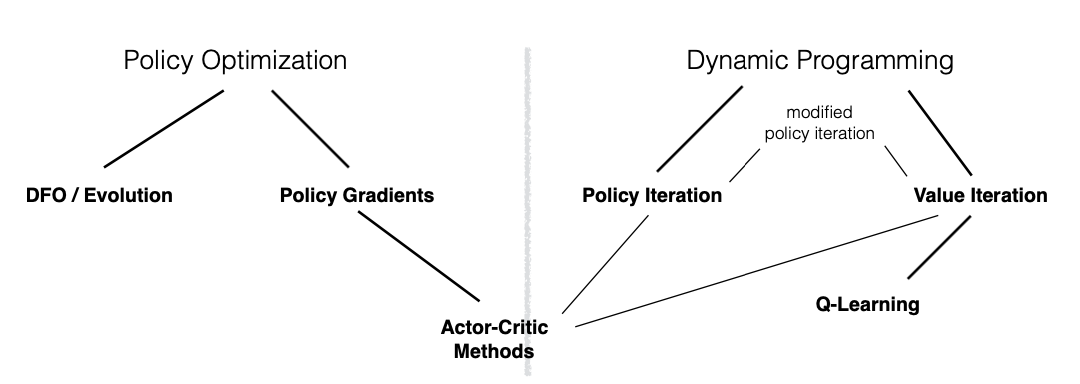
\includegraphics[scale=0.80]{ch3-rl/rf-solve-methods-schulman-thesis-img.png}
    \captionsetup{width=\textwidth} % set the width of the caption
    \caption{Illustration of a taxonomy of model-free RL algorithms. \textbf{Source:} \href{https://rail.eecs.berkeley.edu/deeprlcourse/}{Optimizing Expectations: From Deep Reinforcement Learning to Stochastic Coomputation Graphs} by John, Schulman (2016) \cite{schulman2016optimizing}.}
    \label{fig:rl-model-free-taxonomy}
  \end{figure}

Represent the agent with a function approximator, and we will use a deep neural network for it. That's the reason why are people that call this subfield of reinforcement learning Deep Reinforcement Learning...

The policy is a distributions over actions spawned conditional the states.

\textbf{TODO:} Introduce what we want to maximize, the expected return of the trajectory, and the gradient estimation via score function.

\subsection{Learning the Policy}

The starting point is to think of trajectories as units of learning instead of individual observations (i.e., actions). What dynamics generate a trajectory? 
Given a policy $\pi_{\theta}$, represented as a function with parameter $\theta$, we can deploy the agent into its environment at an initial state $s_0$ and observe its actions in inference mode or \textit{evaluation phase}. The agent continuously promotes actions based on the current state $s_{t}$
until the episode ends in a terminal state, when $t=T$. At this point, we can determine if the goal was accomplished, such as winning the ATARI Pong game, achieving stability in drone flight given the initial settings, \textit{or generating aesthetically pleasing samples from a diffusion model}. The reward signals indicate whether we have achieved the ultimate goal, effectively acting as a ``proxy label'' for the overall trajectory. The return function aggregates the rewards obtained during the trajectory into a single scalar that measures the degree of success of the agent actions. Thus, the trajectory serves as our unit of learning, and the remaining task is to establish the feedback mechanism for the \textit{learning phase}. \\

\noindent Mathematically, we aim to perform stochastic optimization to learn the agent’s parameters. This involves obtaining gradient information from sample trajectories based on performance assessed by a scalar-value function (i.e., reward). The optimization is stochastic because both the agent and environment contain elements of randomness. Therefore, we can only compute estimates of the reward trajectory and gradient. To address this, we use Monte Carlo Gradient Estimation \citep{mohamed2020monte}. It is important to note that from a machine learning perspective, we are performing a double optimization: one due to the stochasticity of the samples for gradient estimation, and the other for the gradient descent algorithms used to update the parameters.

\subsection{Gradient Estimation via Score Function}

The gradient estimation can be obtained using the score function gradient estimator. Let's introduce the following probability objective $\mathcal{F}$, defined in the \href{https://en.wikipedia.org/wiki/Ambient_space_(mathematics)}{ambient space} $\mathcal{X}\in\mathbb{R}^n$ and with parameters $\theta\in\mathbb{R}^n$,

\begin{equation}\label{eqn:probability-objective}
\mathcal{F}(\theta) = \int_{\mathcal{X}} p(\mathrm{x; \theta})f(\mathrm{x})~d\mathrm{x} = \mathbb{E}_{p(\mathrm{x};\theta)}\big[f(\mathrm{x})\big]
\end{equation}

\noindent Here, $f$ is a scalar-valued function, similar to how the reward is represented in the reinforcement learning setting. The \textit{score function} is the derivative of the log probability distribution $\nabla_{\theta}\log p(\mathrm{x};\theta)$ with respect to its parameters $\theta$. We
can use the following identity to establish a connection between
the score function and the probability distribution $p(\mathrm{x};\theta)$.

\begin{equation}\label{eqn:log-derivative-trick-expression}
    \begin{split}
        \nabla_\theta\log p(\mathrm{x};\theta) &= \frac{\nabla_{\theta}p(\mathrm{x}; \theta)}{p(\mathrm{x};\theta)} \\
        p(\mathrm{x};\theta) \nabla_{\theta}\log p(\mathrm{x};\theta) &= \nabla_{\theta}p(\mathrm{x};\theta)
    \end{split}
\end{equation}

\noindent Therefore, taking the gradient of the objective $\mathcal{F}(\theta)$ with respect to the the parameter $\theta$, we have

\begin{equation}\label{eqn:score-function-gradient-objective}
    \begin{split}
        \eta = \nabla_{\theta} \mathbb{E}_{p(\mathrm{x};\theta)}[f(\mathrm{x})] &= \nabla_{\theta}\int_{\mathcal{X}} p(\mathrm{x};\theta) f(\mathrm{x}) d\mathrm{x} \\
        &= \int_\mathcal{X} \nabla_{\theta}~p(\mathrm{x}; \theta)f(\mathrm{x})d\mathrm{x} \\
        &= \int_{\mathcal{X}}p(\mathrm{x};\theta)\nabla_{\theta}\log p(\mathrm{x}; \theta) f(\mathrm{x})d\mathrm{x} \\
        &=\mathbb{E}_{p(\mathrm{x};\theta)}\big[f(\mathrm{x})\nabla_{\theta}\log p(\mathrm{x};\theta) \big] 
    \end{split}
\end{equation}

\noindent The use of the log-derivative rule of Equation~\ref{eqn:log-derivative-trick-expression} to introduce the score function in Equation~\ref{eqn:score-function-gradient-objective} is also known as the \href{https://blog.shakirm.com/2015/11/machine-learning-trick-of-the-day-5-log-derivative-trick/}{\textit{log-derivative trick}}. Now, we can compute an estimate of the gradient, $\bar{\eta}$, using Monte Carlo estimation with samples from the distribution $p(\mathrm{x};\theta)$ as follows:

\begin{equation}\label{eqn:score-function-gradient-estimator}
    \bar{\eta}_{N} = \frac{1}{N}\sum_{i=1}^{N}f\big(\hat{\mathrm{x}}^{(i)}\big) \nabla_{\theta}\log p\big(\hat{\mathrm{x}}^{(i)};\theta\big)
\end{equation}

\noindent We draw $N$ samples $\hat{\mathrm{x}}\sim p(\mathrm{x};\theta)$, compute the gradient of the log-probability for each sample, and multiply by the scalar-valued function $f$ evaluated at the sample. The average of these terms is an unbiased estimate of the gradient of the objective $\eta$, which we can use for gradient ascent, along with a learning rate $\alpha$ to control the step size of the optimization process. The update rule for the parameter $\theta$ is as follows:

\begin{equation}\label{eqn:gradient-ascent}
    \theta \leftarrow \theta + \alpha \bar{\eta}_{N}
\end{equation}

\noindent There are two important points to mention about Equation~\ref{eqn:score-function-gradient-estimator}.

\begin{enumerate}
    \item The function $f$ can be any arbitrary function we can evaluate on $\mathrm{x}$. Even if $f$ is not differentiable with respect to $\theta$, it can still be used to compute the gradient estimation $\bar{\eta}$.
    \item The expectation of the score function is zero, meaning: 
    \begin{equation}\label{eqn:score-function-expectation-zero}
    \begin{split}
        \mathbb{E}_{p(\mathrm{x};\theta)}\big[\nabla_{\theta}\log p(\mathrm{x};\theta)\big] 
        &= \int_{\mathcal{X}}p(\mathrm{x};\theta)\nabla_{\theta}\log p(\mathrm{x}; \theta) d\mathrm{x} \\
        &= \int_{\mathcal{X}} p(\mathrm{x};\theta)\frac{\nabla_{\theta} p(\mathrm{x}; \theta)}{p(\mathrm{x};\theta)}d\mathrm{x} \\
        &= \int_{\mathcal{X}}\nabla_{\theta}p(\mathrm{x};\theta)d\mathrm{x} \\
        &= \nabla_{\theta}\int_{\mathcal{X}} p(\mathrm{x}; \theta)d\mathrm{x} = \nabla_{\theta} 1 =0
    \end{split}
    \end{equation}
\end{enumerate}

\noindent The last point is particularly useful because we can replace $f$ with a shifted version given a constant $\beta$, and obtain the following unbiased estimate of the gradient, which can be beneficial for the optimization task.

\begin{equation}\label{eqn:score-function-gradient-estimator-baseline}
\bar{\eta}_{N} = \mathbb{E}_{p(\mathrm{x}_{\theta})}\big[(f(\mathrm{x}) - \beta) \nabla_{\theta} \log p(\mathrm{x}; \theta)\big]
\end{equation}

\noindent Using a \textbf{\textit{baseline function}} to determine $\beta$ that does not depend on the parameter $\theta$ can reduce the variance of the 
estimator. The baseline function, which satisfies the property in Equation~\ref{eqn:score-function-expectation-zero}, can be any function independent of
$\theta$. When a baseline is chosen to be close to the scalar-valued function $f$, it effectively reduces the variance of the estimator. This reduction in variance helps stabilize the updates by minimizing fluctuations in the gradients estimates, leading to more reliable and efficient learning.

\section{Vanilla Policy Gradient, aka REINFORCE}

The REINFORCE algorithm \citep{williams1992simple} translates the previous 
derivation of gradient estimation via the score function into reinforcement learning terminology. This is the earliest member of the Policy Gradient family (Figure~\ref{fig:rl-model-free-taxonomy}), where the objective is to maximize the expected return of the trajectory $\tau$ under a policy $\pi$ parameterized by $\theta$ (e.g., a neural network). At each state $s_{t}$, the agent takes an action $a_{t}$ according to the policy $\pi$, which generates a probability distribution over actions $\pi(a_{t}\mid s_{t};\theta)$. Here, we will use the notation $\pi_{\theta}(\cdot)$ instead of $\pi(\cdot;\theta)$. \\

\noindent As we mentioned in previous section, a trajectory $\tau$ represents the sequence of state-action pairs resulting from the agent's interaction with its environment. From the initial state $s_{0}$ to the terminal state $s_{T}$, the trajectory $\tau$ is a sequence of states and actions, $\tau = (s_{0}, a_{0}, \dots, s_{T-1}, a_{T-1}, s_{T})$, which describes how the agent
acts during the episodic task. Let $p_{\theta}(\tau)$ be the
probability of obtaining the trajectory $\{\tau^{(i)}\}_{0:T}$ under the policy $\pi_{\theta}$. \\

\noindent We thus have a distribution of trajectories. Recall that the unit of learning is the trajectory $\tau$, and the goal is to maximize the expected return of the trajectory. The return $R(\tau)$ could be the cumulative rewards obtained during the \textit{episode} or the discounted rewards. The expected return is given by the following expression:

\begin{equation}\label{eqn:rl-objective}
    \mathcal{J}(\theta)=\mathbb{E}_{\tau\sim p_{\theta}(\tau)}[R(\tau)] 
\end{equation}

\noindent This is the objective we want to maximize, which is a 
particular case of Equation~\ref{eqn:probability-objective} with the
scalar-valued function $f(\tau) = R(\tau)$, representing the return of the trajectory. Let's use the techniques from the previous section to compute the
gradient of the objective in Equation~\ref{eqn:rl-objective} with respect to the policy parameter $\theta$. The gradient estimation is given by:

\begin{equation}\label{eqn:rl-gradient-estimator-vanilla}
    \nabla_{\theta} \mathbb{E}_{\tau\sim p_{\theta}(\tau)}[R(\tau)] = \mathbb{E}_{\tau\sim p_{\theta}(\tau)}\big[R(\tau)\nabla_{\theta}\log p_{\theta}(\tau)\big]
\end{equation}    


\noindent What exactly is $p_{\theta}(\tau)$? Given that the trajectory is a sequence of states and actions, and assuming the Markov property imposed by the MDP, the probability of the trajectory is defined as follows:

\begin{equation}\label{eqn:trajectory-probability-expanded}
    \begin{split}
        p_{\theta}(\tau) &= p_\theta(s_{0}, a_{0}, s_{1}, a_{1}, \dots, s_{T-1}, a_{T-1}, s_{T}) \\
        &= \rho(s_0)~\prod_{t=0}^{T-1} \pi_{\theta}(a_{t}~|~s_{t})~P(s_{t+1}, r_{t}~|a_{t}, s_{t})
    \end{split}
\end{equation}

\noindent In the above expression, $\rho(s_{0})$ denotes the distribution of initial states, while $P(s_{t+1}, r_{t}\mid a_{t}, s_{t})$ represents the transition model, which updates the environment context based on the action $a_{t}$ taken in the current state $s_{t}$. A crucial step in estimating the gradient is computing the logarithm of the trajectory probability. Following this, we calculate the gradient with respect to the policy parameter $\theta$. 

\begin{equation}\label{eqn:trajectory-gradient-score}
    \begin{split}
        \log p_{\theta}(\tau) &= \log \rho(s_0) + \sum_{t=0}^{T-1}\log \pi_{\theta}(a_{t}~|~s_{t}) + \log P(s_{t+1}, r_{t}\mid a_{t}, s_{t}) \\
        \nabla_{\theta}\log p_{\theta}(\tau) &= \log \cancel{\nabla_{\theta}\rho(s_0)} + \sum_{t=0}^{T-1}\nabla_{\theta}\log \pi_{\theta}(a_{t}\mid s_{t}) + \log\cancel{\nabla_{\theta} P(s_{t+1}, r_{t}\mid a_{t}, s_{t})} \\
        \nabla_{\theta} \log p_{\theta}(\tau) &=  \sum_{t=0}^{T-1}\nabla_{\theta}\log \pi_{\theta}(a_{t}\mid s_{t}) 
    \end{split}
\end{equation}

\noindent The distribution of initial states and the transition
probabilities are disregarded because they are independent of $\theta$, thereby simplifying the computations needed for gradient estimation. By substituting the final expression from Equation~\ref{eqn:trajectory-gradient-score} into the gradient estimation of the objective in Equation~\ref {eqn:rl-gradient-estimator-vanilla}, we derive the REINFORCE gradient estimator.

\begin{equation}\label{eqn:reinforce-gradient-estimator}
    \nabla_{\theta}\mathbb{E}_{\tau\sim p_{\theta}(\tau)}[R(\tau)] = \mathbb{E}_{\tau\sim p_{\theta}(\tau)}\bigg[R(\tau)\bigg(\sum_{t=0}^{T-1} \nabla_{\theta}\log \pi_{\theta} (a_t~|~s_t) \bigg)\bigg] 
\end{equation}

\noindent The core concept is to collect a set of trajectories $\mathcal{D}$ 
by running the policy $\pi_{\theta}$ and update the policy parameters $\theta$ to increase the likelihood of high-reward trajectories while decreasing the likelihood of low-reward ones, as illustrated in Figure~\ref{fig:anatomy-rl-trajectories}. This trial-and-error learning approach, described in Algorithm~3, repeats this process over multiple iterations, reinforcing successful trajectories and discouraging unsuccessful ones, thus encoding the agent's behavior in its parameters. \\

% L3 Foundations of Deep RL series (Pieter  Abbeel)
% https://youtube.com/watch?v=AKbX1Zvo7r8
\noindent \textbf{Reduce the variance of the estimator}. Using two techniques,
\textit{reward-to-go} (aka temporal structure) and \textit{baseline}, we can improve the quality of the gradient estimator in Equation~\ref{eqn:reinforce-gradient-estimator}. \ca{Video de L3 / Abbeel}

\begin{figure}[ht]
    \centering
    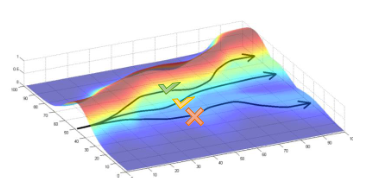
\includegraphics[scale=0.85]{ch3-rl/simulated-trajectories-levine-slides.png}
    \captionsetup{width=\textwidth} % set the width of the caption
    \caption{\textbf{Illustration of three simulated trajectories}, denoted as $\{\tau^{(i)}\}$ where $i=(1,2,3)$, traversing the parametric space $\theta\in\mathbb{R}^2$ under the policy $\pi_{\theta}$. Each trajectory is marked with a colored symbol (cross, check) representing its \textit{goodness} based on the reward function $R(\tau^{(i)})$. \textbf{Source:} \href{https://rail.eecs.berkeley.edu/deeprlcourse/}{Policy Gradients Lecture, Deep Reinforcement Learning Course} by Sergey Levine.}
    \label{fig:anatomy-rl-trajectories}
  \end{figure}
  
% algoritmo naive REINFORCE
\begin{algorithm}
    \caption{Vanilla Policy Gradient, aka REINFORCE}
    \begin{algorithmic}
    \STATE Initialize policy $\pi_{\theta}$, set learning rate $\alpha$
    % \STATE Generate $\tau=(s_0, a_0, ..., s_{T-1}, a_{T-1}, s_{T})$ by sampling from current $\pi_{\theta}$
    \FOR {$\text{iteration}=0, 1, 2, \dots, N$}
        \STATE Collect a set of trajectories $\mathcal{D}=\{\tau^{(i)}\}_{0:T-1}$ by sampling from the current policy $\pi_{\theta}$
        \STATE Calculate the returns $R(\tau^{(i)})$ for each trajectory $\tau^{(i)}$
        \STATE Update the policy: $\theta \leftarrow \theta + \alpha \bigg(\frac{1}{|\mathcal{D}|(T-1)}\sum_{\tau^{(i)}\in\mathcal{D}}\sum_{0}^{T-1}\nabla_{\theta}\log\pi_{\theta}(a_{t}\mid s_{t})R(\tau^{(i)})\bigg)$
    \ENDFOR
    \end{algorithmic}
\end{algorithm}

\noindent \ca{Aca reward-to-go y explicar idealmente prque menos terminos reduce la varianza} A naive estimate of $R(\tau)$ uses the total trajectory reward, which means that every action is weighted by the total reward. Even if the gradient estimator is unbiased, we need to consider the variance of the estimator.
To reduce this variance, we can impose causality by using rewards-to-go, i.e., the sum of rewards from the current time-step to the end of the trajectory. This simple trick can reduce variance. 

\begin{equation}\label{eqn:reinforce-gradient-reward-to-go}
    \nabla_{\theta}\mathbb{E}_{\tau\sim p_{\theta}(\tau)}[R(\tau)] = \mathbb{E}_{\tau\sim p_{\theta}(\tau)}\bigg[\bigg(\sum_{t=0}^{T-1} \nabla_{\theta}\log \pi_{\theta} (a_t~|~s_t)\bigg) \bigg(\sum_{t'=t}^{T-1}R(s_{t}, a_{t}, s_{t+1})\bigg)\bigg] 
\end{equation}

\noindent Notice that the sum of the reward index is dependent on $t$. For action $t$, we  will weight rewards from $t$ to $T-1$; for action $t+1$, we will weight rewards from $t+1$ to $T-1$, and so on. There is no effect of previous rewards on the weight of the current action; only the consequence of the current action on the future rewards matters. This is the causality we want to impose in the gradient estimator \ca{Mejorar este parrafo para entender bien consecuencias del reward to go e idealmente como se deriva...}. \\

\noindent As we see in the previous section, it is possible to reduce the
variance of the gradient estimator by using a baseline function, $b(s_{t})$, without biasing the estimator, i.e., at no additional cost. However, is the expectation of the score still unbiased in this setting? 

\begin{equation}\label{eqn:reinforce-gradient-estimator-baseline}
    \begin{split}
        \nabla_{\theta}\mathbb{E}_{\tau\sim p_{\theta}(\tau)} &= \mathbb{E}_{\tau\sim p_{\theta}(\tau)} \bigg[\sum_{t=0}^{T-1}\nabla_{\theta}\log\pi_{\theta}(a_{t}|s_{t}) \bigg( \sum_{t=t'}^{T-1} r_{t'}-b(s_{t}) \bigg) \bigg]
    \end{split}
\end{equation}

\noindent The proof follows a similar argument as shown in Equation~\ref{eqn:score-function-expectation-zero}, with the key difference being that the expectation is taken with respect $p_{\theta}(\tau)$, which is a sequence of random variables. By leveraging the linearity of the expectation property, we can focus on a single term at step $t$ of Equation~\ref{eqn:reinforce-gradient-estimator-baseline} to demonstrate that the baseline does not affect the expectation of the score function. We split the trajectory sequence $\tau$ at step $t$ into: $\tau_{0:t}$ and $\tau_{t+1:T-1}$, and then expand it into state-action pairs\footnote{A criterion used when splitting the trajectory is that state-action pairs are formed given that $s_{t}$ is a consequence of action $a_{t-1}$, and taking action $a_{t}$ results in state $s_{t+1}$. Notice both expectations from step 1 and 2 in Equation~\ref{eqn:reinforce-baseline-unbiased}.}.

\begin{equation}\label{eqn:reinforce-baseline-unbiased}
   \begin{split}
        \mathbb{E}_{\tau\sim p_{\theta}(\tau)}\big[\nabla_{\theta}\log\pi_{\theta}(a_t|s_t) b(s_t) \big] &=  \mathbb{E}_{\tau_{(0:t)}}\big[\mathbb{E}_{\tau_{(t+1:T-1)}}[ \nabla_{\theta}\log \pi_{\theta}(a_{t}|s_{t})b(s_{t})]\big]  \\
        &= \mathbb{E}_{s_{0:t}, a_{0:t-1}}\big[\mathbb{E}_{s_{t+1:T}, a_{t:T-1}}[ \nabla_{\theta}\log \pi_{\theta}(a_{t}|s_{t})b(s_{t})]\big] \\
        &= \mathbb{E}_{s_{0:t}, a_{0:t-1}}\big[b(s_{t})\mathbb{E}_{s_{t+1:T}, a_{t:T-1}}[ \nabla_{\theta}\log \pi_{\theta}(a_{t}|s_{t})]\big] \\
        &= \mathbb{E}_{s_{0:t}, a_{0:t-1}}\big[b(s_{t})\mathbb{E}_{a_{t}}[ \nabla_{\theta}\log \pi_{\theta}(a_{t}|s_{t})]\big] \\
        &= \mathbb{E}_{s_{0:t}, a_{0:t-1}}\big[b(s_{t})\nabla_{\theta}\mathbb{E}_{a_{t}}[\log \pi_{\theta}(a_{t}|s_{t})]\big] \\
        &= \mathbb{E}_{s_{0:t}, a_{0:t-1}}\big[b(s_{t})\nabla_{\theta}1\big] \\
        &= 0
   \end{split}
\end{equation}

\noindent We can remove irrelevant variables from the expectation over the portion of the trajectory $\tau_{(t+1):(T-1)}$ because we are focusing on the term at step $t$. The only relevant variable is $a_{t}$, and the expectation $\mathbb{E}_{a_{t}}\log\pi_{\theta}(a_{t}\mid s_{t})$ is 1. Given that the
gradient with respect to $\theta$ of a constant is zero, and $b(s_{t})$ is multiplying it, the effect of the baseline on the expectation is nullified. This argument can be applied to any other term in the sequence due to the linearity of the expectation. Therefore, we have proven that using a baseline also keeps the gradient estimator unbiased in the policy gradient setting. \\

\noindent \textbf{What baseline to use?} Estimate the \textit{advantage function} $A_{t} = \sum_{t=0}^{T-1} r_{t}^{'}-b(s_{t})$...\ca{\textbf{TODO:} introducir términos para (i) $R(\tau)$ y (ii) $b(s_{t})$. Además especificar que el uso de MSE loss para ajustar state-value function que se usa como baseline...}

\begin{algorithm}
    \caption{REINFORCE with advantage \ca{\textbf{TODO:} terminar de detallar este algoritmo...}}
    \begin{algorithmic}
    \STATE Initialize policy $\pi_{\theta}$, set learning rate $\alpha$
    \STATE Initialize a value $V_{\phi}$
    \FOR {$\text{iteration}=0, 1, 2, \dots, N$}
        \STATE Collect a set of trajectories $\mathcal{D}=\{\tau^{(i)}\}_{0:T-1}$ by sampling from the current policy $\pi_{\theta}$
        \STATE Calculate the returns $R(\tau^{(i)})$ for each trajectory $\tau^{(i)}$
        \STATE Update the policy: $\theta \leftarrow \theta + \alpha \bigg(\frac{1}{|\mathcal{D}|(T-1)}\sum_{\tau^{(i)}\in\mathcal{D}}\sum_{0}^{T-1}\nabla_{\theta}\log\pi_{\theta}(a_{t}\mid s_{t})R(\tau^{(i)})\bigg)$
        \STATE Update the value: $\phi \leftarrow \phi + \alpha \bigg(\frac{1}{|\mathcal{D}|(T-1)}\sum_{\tau^{(i)}\in\mathcal{D}}\sum_{0}^{T-1}\nabla_{\phi}V_{\phi}(s_{t})\bigg)$
    \ENDFOR
    \end{algorithmic}
\end{algorithm}



% \noindent \ca{Terminar esta parte...} We know that introducing a baseline keeps the estimator unbiased, but why the baseline can reduce the variance of the estimator? In \cite{seita2017going} there is an explanation of how to rearrange the variance of the score function and queda formulado una esperanza factorizada donde esta el retorno menos el baseline. De poder optimizarse, se puede formular como least square error, y la función de baseline ideal sería estimar el retorno esperado. Así sabemos si el retorno esta sobre o bajo el retorno esperado, y reduciendo la varianza  del estimador al mismo tiempo...preguntar sobre manipulación de la esperanza y agregar formulación!


\section{Deep Reinforcement Learning}

The REINFORCE algorithm is a simple and powerful algorithm to learn the policy,
even more when we equipped the agent with a neural network as a function 
approximation of the policy. 

\textbf{TODO:} Implement the REINFORCE algorithm in a simple environment, such as ATARI PONG game. Focus to highlight the following:

\begin{enumerate}
    \item The policy is a neural network that takes the state as input and output a distribution over actions, i.e. softmax layer.  
    \item Using automatic differentiation as engine to backpropagate the gradient estimation. We need a loss function to compute the gradient, how
    can we convert the Eq.~\ref{eqn:reinforce-gradient-estimator} into a loss?
    \item Take advantage of neural network to learn useful representations from raw data such as images (e.g. convolutions).
\end{enumerate}

\begin{equation}\label{eqn:neural-softmax-policies}
    \pi_{\theta}(a~|~s) = \frac{\exp(f_{\theta}(s, a))}{\sum_{a'\in\mathcal{A}}\exp(f_{\theta}(s, a'))}
\end{equation}

\noindent In the previous section we see how to get an expression to estimate the gradients. However, in practice, where we use complex function
$f_{\theta}$ to approximate our policy $\pi$, we want to express a cost
function $\mathcal{J}(\theta)$ in a manner that we can take advantange of 
automatic differentiation engines such as PyTorch or JAX.

\begin{equation}\label{eqn:reinforce-gradient-estimator-cost}
    \mathcal{J}(\theta) = \mathbb{E}_{p_{\theta}(\tau)}\bigg[R(\tau)\bigg(\sum_{t=0}^{T-1} \log \pi_{\theta} (a_t~|~s_t) \bigg)\bigg] 
\end{equation}

\noindent We will use a convolutional neural network design to learn features from raw input such as RGB images or video frames. Without any prior information about the ATARI game more than the inductive bias of the neural network tailord to process images, we will learn a policy that maximize the reward, i.e., win the game. \\

% \noindent The preprocessing regarding the raw Atari images is from $210\times 160$ pixel images

\noindent Regarding the preprocessing of the raw Atari images, we follow the instructions
from the work playing atari games \cite{mnih2013playing}. It consist in
apply to the $210\times 160$ images a 2 factor down-samplig to $110\times 84$
and from RGB to grayscale. The resulted images were cropped into a $84\times84$
region of the pixels that represent the ``playing area''.

\section{Improving Sample Efficiency: Behavior and Target Policies}

% \ca{Util de referencia en literatura \cite{peshkin2002learning}}

The main drawback of the REINFORCE algorithm is its sample complexity. Once we roll out the policy and collect the data, we cannot reuse it after the policy has been updated. We must collect new data following the \textit{target policy} $\pi_{\theta}$ that we want to update. In RL literature, this is referred to as \textit{on-policy} learning. Reusing the data $\mathcal{D}\sim\pi_{\theta_{\text{old}}}$ to update the current policy $\pi_{\theta}$ would significantly improve sample efficiency. However, once we update the policy, the previously collected data is no longer valid because the policy has changed. The distribution from which the data was sampled is now $\pi_{\theta_{\text{old}}}$. \\

\noindent Using behavior data learned from another policy, known as a \textit{behavior policy}, to update the current policy is referred to as \textit{off-policy} learning in RL literature. Let's introduce a \textit{behavior policy} in the RL objective defined in Equation~\ref{eqn:rl-objective} using \href{https://timvieira.github.io/blog/post/2014/12/21/importance-sampling/}{importance sampling
}:

% Derive RL objective with importance sampling to use data from another policy
\begin{equation}\label{eqn:derive-rl-objective-with-is}
    \begin{split}
        \nabla_{\theta}\mathcal{J}(\theta) &= \mathbb{E}_{\tau \sim p_{\theta}(\tau)}\bigg[ \nabla_{\theta}\log p_{\theta}(\tau) R(\tau)\bigg] \\
        &= \mathbb{E}_{\tau \sim p_{\theta}(\tau)} \bigg[ \frac{\nabla_{\theta}p_{\theta}(\tau)}{p_{\theta}(\tau)} R(\tau) \bigg] \\
        &= \int_{\mathcal{X}} p_{\theta}(\tau) \frac{\nabla_{\theta}p_{\theta}(\tau)}{p_{\theta}(\tau)} R(\tau) d\tau \\
        &= \int_{\mathcal{X}} \frac{p_{\theta_{\text{old}}}(\tau)}{p_{\theta_{\text{old}}}(\tau)} \cancel{p_{\theta}(\tau)} \frac{\nabla_{\theta}p_{\theta}(\tau)}{\cancel{p_{\theta}}(\tau)} R(\tau) d\tau \\
        &= \int_{\mathcal{X}} p_{\theta_{\text{old}}}(\tau) \frac{\nabla_{\theta}p_{\theta}(\tau)}{p_{\theta_{\text{old}}}(\tau)} R(\tau) d\tau \\
        &= \mathbb{E}_{\tau\sim p_{\theta_{\text{old}}}(\tau)} \bigg[\frac{\nabla_{\theta} p_{\theta}(\tau)}{p_{\theta_{\text{old}}}(\tau)} R(\tau)\bigg]
    \end{split}
\end{equation}

\noindent We derive a new objective that is more general and reconciles both \textit{on-policy} and \textit{off-policy} learning.

% RL objective with IS
\begin{equation}\label{eqn:rl-objective-with-is}
    \mathcal{J}_{\text{IS}}(\theta) = \mathbb{E}_{\tau\sim p_{\theta_{\text{old}}}(\tau)}\bigg[\frac{p_{\theta}(\tau)}{p_{\theta_{\text{old}}}(\tau)} R(\tau)\bigg]
\end{equation}

\noindent We can assume that the data collected from the behavior policy is
not so different from the target policy, and use first order approximation to
update the policy. 

\begin{equation}\label{eqn:rl-objective-is-linear-aprox}
    \begin{split}
        \nabla_{\theta}\mathcal{J}(\theta)\rvert_{\theta=\theta_{\text{old}}} &= \mathbb{E}_{\tau\sim p_{\theta_{\text{old}}}(\tau)} \bigg[\frac{\nabla_{\theta} p_{\theta}(\tau)\rvert_{\theta=\theta_{\text{old}}}}{p_{\theta_{\text{old}}}(\tau)} R(\tau)\bigg] \\
        &= \mathbb{E}_{\tau\sim p_{\theta_{\text{old}}}(\tau)} \big[\nabla_{\theta}\log p_{\theta}(\tau)\rvert_{\theta=\theta_{\text{old}}} R(\tau) \big]
    \end{split}
\end{equation}


\noindent \textbf{The problem with first order approximation}. The gradient estimation it is good only in the inmediate vecinity, because is a local approximation of the function. Hence, the step size is crucial to avoid a policy degradation, a situation where the policy is updated with a bad gradient,
it is difficult to recover from this situation. Given that the data is collected by the policy, the feedback loop can be dangerous for the training
stability. \\

\section{Trust Region and Proximal Policy Optimization}

\ca{Agregar función objetivo...de Costa Huang. Paper TRPO \cite{schulman2015trust} y PPO \cite{schulman2017proximal}}

% See [Schulman 2015 \cite{schulman2015trust}], section 3.10 with the proof.


Show a high level overview of TRPO (Pieteer Abbel L4). Make efficient use of data (compare with classic PG). The core idea is the policy in a way that ``improve a certain surrogate objective as much as possible, while changing the policy as little as possible, where this is change is measured as a KL divergence between action distributions.'' Trut region 
is a region where the policy is close to the old policy and we can achieve this constraint improvement.

Then, PPO simplify objective to avoid a second-order optimization, showing
good results and be the de-facto standard in RL \cite{dlr191986}. 


% algoritmo naive REINFORCE
\begin{algorithm}
    \caption{Proximal Policy Optimization (PPO)}
    \begin{algorithmic}
    \STATE Initialize policy parameter $\theta$, set learning rate $\alpha$
    \STATE Generate $\tau=(s_0, a_0, ..., s_{T-1}, a_{T-1}, s_{T})$ by sampling from current $\pi_{\theta}$
    \FOR{$t=0, 1, \dots, T-1$}
        \STATE Estimate the return $R(\tau)$
        \STATE Update the policiy parameters $\theta \leftarrow \theta + \alpha~r_{t}\nabla_{\theta}\log\pi_{\theta}(a_{t}|s_{t})$
    \ENDFOR
    \end{algorithmic}
\end{algorithm}



\section{Reinforcement Learning From Human Feedback}

In this section we will brielfy put in context what the hell is RLHF.
For design and train reward model we refer to XYZ.


\section{Summary}

In a summary, solve a reinforcement learning problem
via proximal policy...